% Sample file: amsart.tpl
%BEGIN_FOLD
% Preamble
\documentclass[12pt, a4paper, reqno]{amsart}
\usepackage{amssymb,latexsym}
\usepackage{amsthm}
\usepackage{fontspec} % For font settings
\usepackage{xeCJK} % Package for Chinese support
\usepackage{tikz}
\usepackage{esvect} %向量长箭头
\usepackage{geometry} % Add this package to set the page dimensions
\usepackage{graphicx}
\usepackage{caption} % 图片caption
\usepackage[colorlinks=true, linkcolor=blue]{hyperref}% 超链接或references
\usepackage{romannum} % 罗马数字
\usepackage{chngcntr} % Package to change counters

% Set the page margins to make the content wider and text centered horizontally
\geometry{
	left=2.5cm,   % Left margin, smaller values = wider text
	right=2.5cm,  % Right margin, smaller values = wider text
	top=1.75cm,    % Top margin
	bottom=1.75cm, % Bottom margin
	includehead, % Includes space for the header within the specified margin
	includefoot  % Includes space for the footer within the specified margin
}

\renewcommand{\arraystretch}{1.5} % 行高1.5倍

% Redefine the theorem style to be non-italic for all theorem-like environments
\theoremstyle{definition}
\newtheorem{theorem}{Theorem}[subsection] % Non-italic theorem, numbered within sections
\newtheorem{lemma}[theorem]{Lemma}      % Non-italic lemma, shares numbering with theorem
\newtheorem{corollary}[theorem]{Corollary}  % Non-italic corollary, shares numbering with theorem
\newtheorem{definition}[theorem]{Definition} % Non-italic definition, shares numbering with theorem
\newtheorem{example}{Example}[subsection] % Non-italic example, independently numbered within sections


\newtheorem*{definition*}{Definition} % Unnumbered definitions non-italic
\newtheorem*{theorem*}{Theorem}

\numberwithin{equation}{section} % Equations numbered within sections

% Redefine the footnote numbering format
\renewcommand{\thefootnote}{\thesection.\arabic{footnote}}

% Ensure footnotes reset at each section
\counterwithin{footnote}{section}


% Set Chinese font (adjust the font name as needed)
\setCJKmainfont{SimSun} % Use a common Chinese font such as SimSun, or another you have installed
% Customize caption font size
%\captionsetup{font=small}
\captionsetup{font=scriptsize} % For scriptsize captions


\DeclareMathOperator{\arccot}{arccot} % Define arccot function
%END_FOLD
\begin{document}
%BEGIN_FOLD
% One author
\title{Chapter 9 Vectors}
%\author{name}
%\address{line1\\
%         line2\\ 
%         line3} 
%\email{name@address}
%\urladdr{http://webaddress}
%\thanks{thanks}

% End one author



%\keywords{keywords}
%\subjclass[2010]{Primary: subject; Secondary: subject}
%\date{date}
%
%\begin{abstract}
%   abstract
%\end{abstract}
\maketitle
%END_FOLD

\section{Vectors: Geometric View}\label{S:VGV}

\subsection{Definition of Vectors}\label{SS:DOV}

\begin{definition}\label{D:VEC} \textbf{(Vectors)}
	Quantities has both a \textbf{magnitude} (the ``how much" or ``how big" part) and a \textbf{direction} in space are called vectors. Magnitude of a vector is also called \textbf{norm} or \textbf{length}.
\end{definition}

On notation of vectors, different books or authors have different habits, you may see $\textbf{A}\text{ (boldface letter)}, \vv{A}\text{ (with an arrow above)}, \vv{\textbf{A}}\text{ (two ways together)}$ etc. I will stick to $\vv{A}$, because I like using boldface letter to make readers to pay attention to those words. Formally we have:
\begin{itemize}
	\item position vector of point A which starts at the origin: $\vv{OA}$, we denote its magnitude as $\left|\vv{OA}\right|$\footnote{Some books might use the symbol $\left\|\vv{OA} \right \|$ for the magnitude of a vector.}\label{f:norm} or $OA$.
	\item displacement vector of B relative to A: $\vv{AB}$, its length $\left|\vv{AB}\right|$
\end{itemize}

Finally, we say \textbf{two vectors are equal} if they have the same magnitude and direction, and \textbf{the negative of a vector $\vv{a}$} is the vector parallel to $\vv{a}$ and with the same length, but in the opposite direction. It is denoted $-\vv{a}$.


\subsection{Basic Operations}\label{SS:BO}\hfill

In this part, I want to briefly talking about vector addition (subtraction) and vector multiplied by a scalar. As this is just a note, I will only give you some schematic diagram\footnote{The three pictures all come from the book \textit{The Mechanical Universe: Mechanics and Heat} by Steven C. Frautschi, Richard P. Olenick, Tom M. Apostol and David L. Goodstein.}\label{f:VAS}:

\begin{minipage}{.5\textwidth}
	\centering
	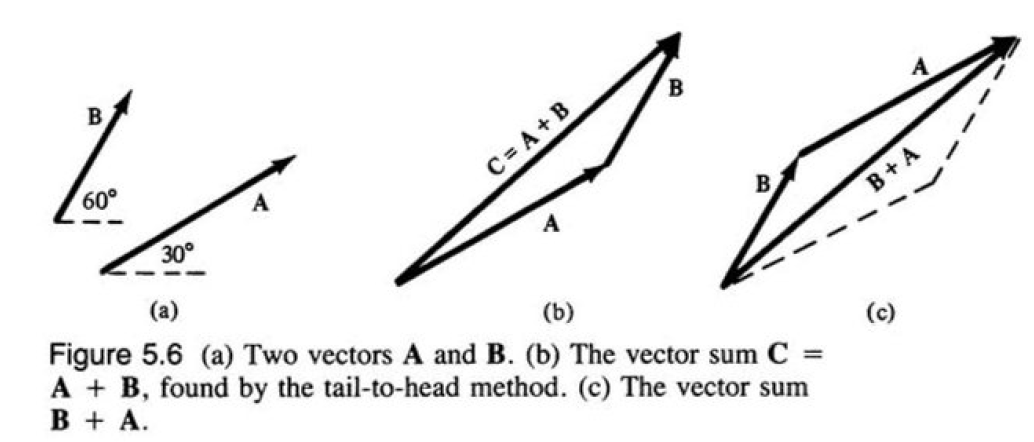
\includegraphics[width=.9\linewidth]{1.png}
	\captionof{figure}{}
	\label{F:ADD}
\end{minipage}%
\begin{minipage}{.5\textwidth}
	\centering
	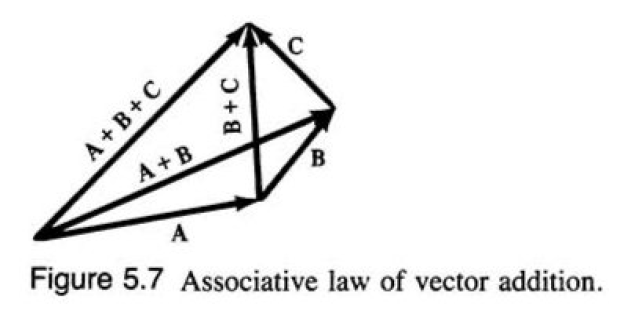
\includegraphics[width=.9\linewidth]{2.png}
	\captionof{figure}{}
\end{minipage}
\begin{figure}[h]
	\centering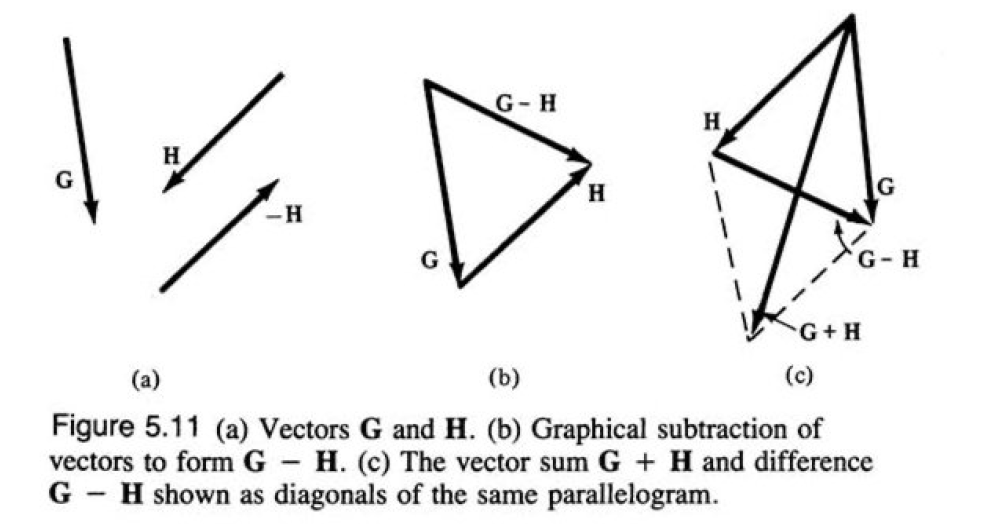
\includegraphics[width=.4\linewidth]{3.png}
	\caption{}
	\label{fig:VAS}
\end{figure}

Pictures above show the way we doing vector addition or subtraction, an interesting fact is that, $\vv{BA}$, which is the sum of two vectors, is a diagonal of a parallelogram. However, as Figure~\ref{fig:VAS} shows, the subtraction is another diagonal.

For a vector multiplied by a scalar, its just a stretching or compressing of the vector, omitted here. But one thing is important:
\begin{theorem}\label{T:PARA} \textbf{(Parallel)}
	Two non-zero vectors are parallel if and only if one is a scalar multiple of the other i.e.
	\begin{equation}\label{E:PARA}
		\vv{a}\parallel \vv{b} \Leftrightarrow \vv{a}=\lambda \vv{b}.
	\end{equation}
\end{theorem}

\subsection{The Scalar Product}\label{SS:TSP}

\begin{definition}\label{D:SP} \textbf{(The Scalar Product)}
	The scalar product, also called dot product or inner product of two vectors, say $\vv{a}, \vv{b}$ is defined as:
	\begin{equation}\label{E:SP}
		\vv{a}\cdot \vv{b} = \left|\vv{a}\right|\left|\vv{b}\right|\cos \theta
	\end{equation}
	Here, $\theta$ is the small angle between the two vectors (ranges from $0$ to $\pi$).
\end{definition}

We have another definition:(forgive my laziness)
\footnote{The source of the figure is \textit{Mathematics Application and Interpretation HL 2} by Michael Haese, Mark Humphries, Chris Sangwin and Ngoc Vo.}
\begin{definition}\label{f:Components} \textbf{(Components)}:
	\begin{figure}[h]
		\centering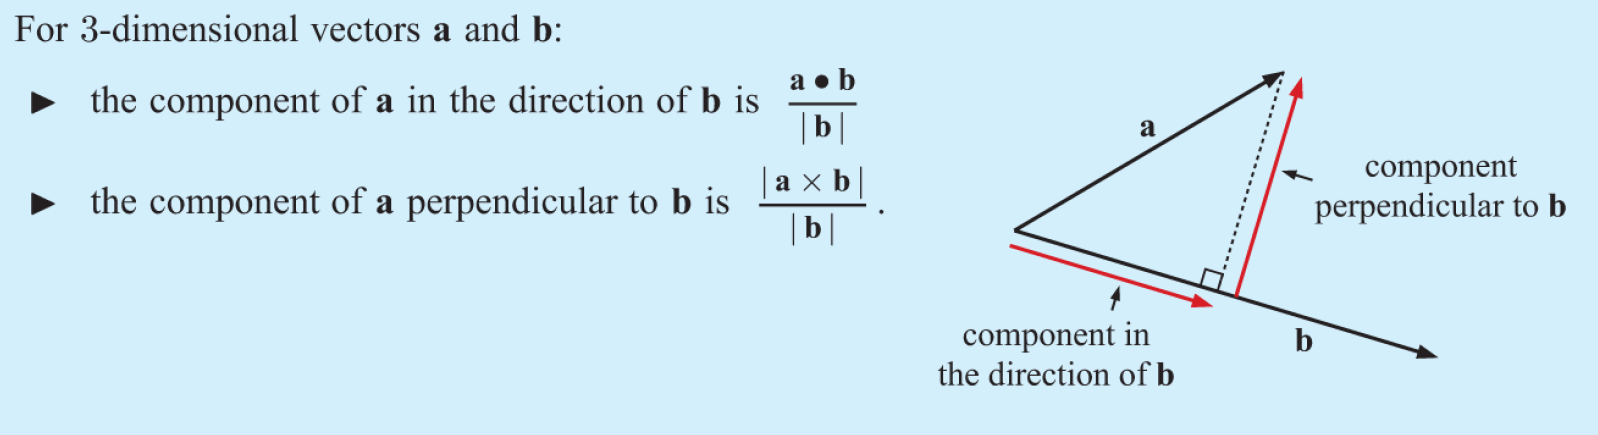
\includegraphics[width=1\linewidth]{14.png}
		\caption{}
	\end{figure}
\end{definition}

Please notice that component is a scalar! If you want the vector along the direction of $\vv{b}$ with magnitude as the component of $\vv{a}$ in the direction of $\vv{b}$, what you are searching for is a concept called projection:
\begin{definition}\label{D:PRJ} \textbf{(Projection)}
	\begin{equation}\label{E:Projection}
		\text{Projection $\vv{a}$ onto $\vv{b}$} = \frac{\vv{a}\cdot \vv{b}}{\left|\vv{b}\right|}\vv{b}
	\end{equation}
\end{definition}

There is an useful schematic diagram for scalar product\footnote{These three pictures comes from \textit{University Physics with Modern Physics} (14th ed.) by Young and Freedman}\label{f:AA}:

\begin{minipage}{.3\textwidth}
	\centering
	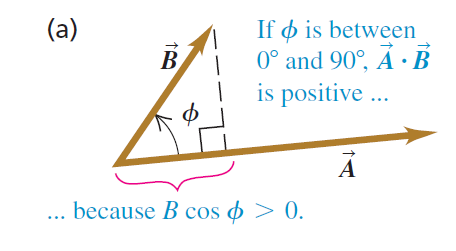
\includegraphics[width=1\linewidth]{4.png}
	\captionof{figure}{}
\end{minipage}%
\begin{minipage}{.3\textwidth}
	\centering
	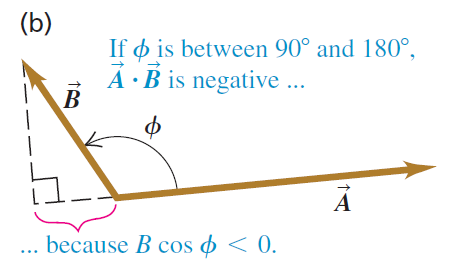
\includegraphics[width=1\linewidth]{5.png}
	\captionof{figure}{}
\end{minipage}
\begin{minipage}{.3\textwidth}
	\centering
	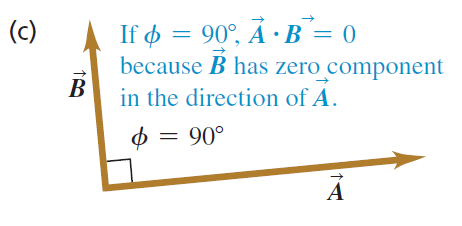
\includegraphics[width=1\linewidth]{6.png}
	\captionof{figure}{}
\end{minipage}%



This shows that the sign of scalar product reveal the angle between two vectors, if the value of scalar product is positive, the angle will be an acute angle, negative for an obtuse angle, 0 for a right angle, actually we have:
\begin{theorem}\label{T:ABV} \textbf{(Angle between Vectors)}
	\begin{equation}
		\cos \theta = \frac{\vv{a}\cdot \vv{b}}{\left|\vv{a}\right|\left|\vv{b}\right|}.
	\end{equation}
\end{theorem}
Some special cases need us to pay more attention:
\begin{theorem}\label{T:PaPoV} \textbf{(Perpendicular and Parallel)}
	\begin{align}
		\vv{a} \perp \vv{b} \Leftrightarrow \vv{a}\cdot \vv{b} = 0\\
		\vv{a} \parallel \vv{b} \Leftrightarrow \left|\vv{a}\cdot \vv{b}\right| = \left|\vv{a}\right|\left|\vv{b}\right|
	\end{align}
\end{theorem}



We will see more application of scalar product when introduction the Cartesian coordinate, just wait and see.

\subsection{The Vector Product}\label{SS:TVP}

\begin{definition}\label{D:TVP} \textbf{(The Vector Product)}
	We denote the vector product of two vectors $\vv{a}, \vv{b}$, also called cross product, by $\vv{a}\times \vv{b}$. The result of it is a vector, and we define it by defining its magnitude and direction:
	\begin{itemize}
		\item magnitude:
		\begin{equation}\label{E:TVP}
			\left|\vv{a}\times \vv{b}\right| = \left|\vv{a}\right|\left|\vv{b}\right|\sin \theta
		\end{equation}
		\item direction: $\vv{a}\times \vv{b}$ is perpendicular to the plane formed by $\vv{a}\text{ and }\vv{b}$, and using the \textbf{right-hand rule} to choose the final direction.
	\end{itemize}
\end{definition}

At first glance, the definition of vector product is kind of complex, but there are also helpful schematic diagrams\footnote{The source of the first two figures are the same as in footnote \ref{f:VAS}, and the source of the last two figures are the same as in footnote \ref{f:AA}.}\label{f:Cross}:

\begin{figure}[h]
	\centering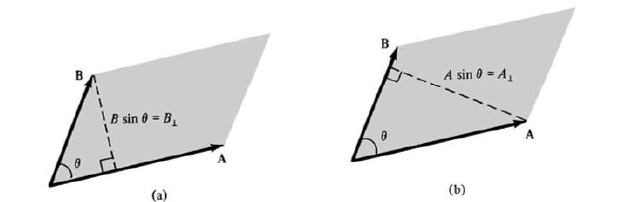
\includegraphics[width=.6\linewidth]{7.png}
	\caption{}
	\label{P:MoVP}
\end{figure}
\begin{minipage}{.5\textwidth}
	\centering
	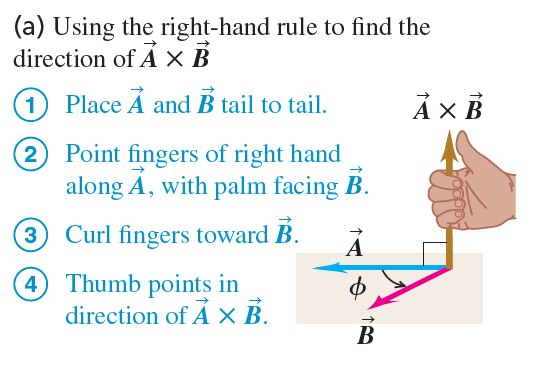
\includegraphics[width=.6\linewidth]{8.png}
	\captionof{figure}{}
	\label{P:AXB}
\end{minipage}%
\begin{minipage}{.5\textwidth}
	\centering
	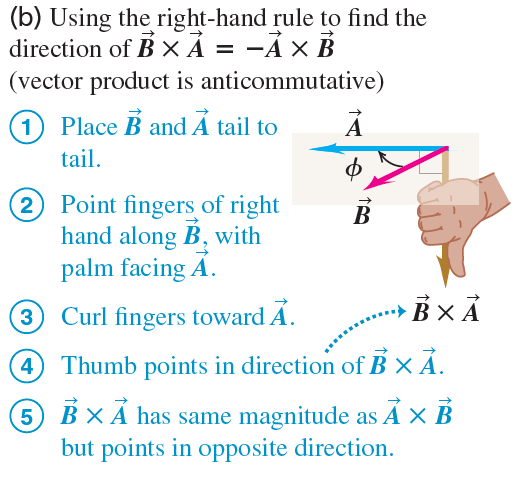
\includegraphics[width=.6\linewidth]{9.png}
	\captionof{figure}{}
	\label{P:BXA}
\end{minipage}

Figure~\ref{P:MoVP} shows that the magnitude of vector product is the area of the parallelogram ``spaned" by the two vectors. Then Figure~\ref{P:AXB} and Figure~\ref{P:BXA} just show you how the right hand rule working. Notice that I have been ignoring the rules of operations of vectors, say like the commutative law of vector addition etc. The reason is that most of them are like the rules for numbers. However, the only difference just showed up, we have:
\begin{theorem}\label{T:AC} \textbf{(Anticommutative Law of Vector Product)}
	\begin{equation}
		\vv{a}\times \vv{b} = - \vv{b}\times \vv{a}
	\end{equation}
\end{theorem}

Vectors can be more applicable, but we have to bring something up here. Don't worry, it is Mr.Descartes comes to help.

\newpage
\section{Vectors with Cartesian Coordinate}\label{S:VCC}

\subsection{Introducing Cartesian Coordinate}\label{SS:ICC}\hfill

I believe the readers have been quite familiar with the Cartesian coordinate system, so I just want to show you two graph of it\footnote{The source of the two figures are the same as in footnote~\ref{f:VAS}}\label{f:CC}:

\begin{minipage}{.5\textwidth}
	\centering
	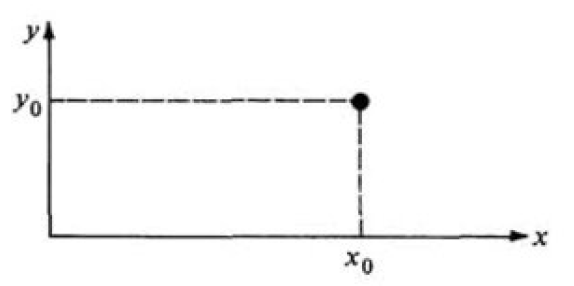
\includegraphics[width=.7\linewidth]{10.png}
	\captionof{figure}{}
\end{minipage}%
\begin{minipage}{.5\textwidth}
	\centering
	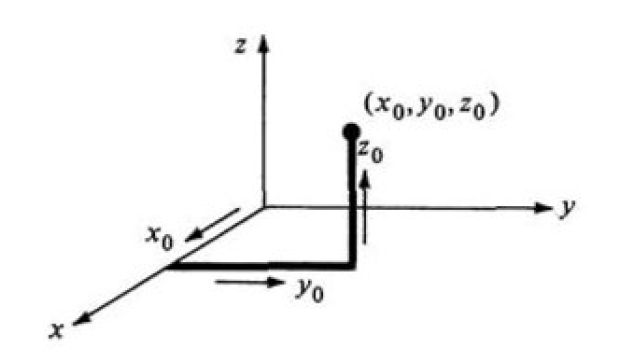
\includegraphics[width=.7\linewidth]{11.png}
	\captionof{figure}{}
\end{minipage}

Here, only a little knowledge needs to be introduced:
\begin{definition}\label{D:ijk} \textbf{(Unit Vector and $\vv{i}, \vv{j}, \vv{k}$)}
	\textbf{A unit vector is a vector that has a magnitude of 1}, its only purpose is to point—that is, to describe a direction in space.
	
	In an xy-coordinate system we can define a unit vector $\vv{i}$\textbf{that points in the direction of the positive x-axis} and a unit vector $\vv{j}$ \textbf{that points in the direction of the positive y-axis}. If we are dealing with a xyz-coordinate, we define a unit vector $\vv{k}$ \textbf{that points in the direction of the positive z-axis}.
	
	\begin{center}
		\begin{minipage}{0.45\textwidth}
			\centering
			\begin{tikzpicture}[scale=0.6]
				% Draw the y-axis with arrow in the middle
				\draw[thick] (-1,0,0) -- (3,0,0) node[right] {$x$};
				\draw[->, thick] (0,0,0) -- (1,0,0) ;
				\node at (1,0,0) [below] {$\vv{i}$};
				
				% Draw the x-axis with arrow in the middle
				\draw[thick] (0,-1,0) -- (0,3,0) node[above] {$y$};
				\draw[->, thick] (0,0,0) -- (0,1,0) ;
				\node at (0,1,0) [right] {$\vv{j}$};
				
				% Draw the origin
				\node at (0,0,0) [below right] {$O$};
			\end{tikzpicture}
			\captionof{figure}{}
		\end{minipage}
		\begin{minipage}{0.45\textwidth}
			\centering
			\begin{tikzpicture}[scale=0.6]
				% Draw the z-axis with arrow in the middle
				\draw[thick] (0,0,0) -- (0,0,3.54) node[above] {$x$};
				\draw[->, thick] (0,0,0) -- (0,0,1.414) ;
				\node at (0,0,1) [left] {$\vv{i}$};
				
				% Draw the y-axis with arrow in the middle
				\draw[thick] (0,0,0) -- (2.5,0,0) node[right] {$y$};
				\draw[->, thick] (0,0,0) -- (1,0,0) ;
				\node at (1,0,0) [below] {$\vv{j}$};
				
				% Draw the x-axis with arrow in the middle
				\draw[thick] (0,0,0) -- (0,2.5,0) node[above] {$z$};
				\draw[->, thick] (0,0,0) -- (0,1,0) ;
				\node at (0,1,0) [right] {$\vv{k}$};
				
				% Draw the origin
				\node at (0,0,0) [below right] {$O$};
			\end{tikzpicture}
			\captionof{figure}{}
		\end{minipage}
	\end{center}
\end{definition}

\subsection{Converting}\label{SS:CVT}\hfill

Now, a critical problem, if we know a vector which means we know its magnitude and direction, how can we represent it in the Cartesian coordinate? Here suppose the meaning of the direction of a vector is denoted by the angle between the vector and x-axis which is $\theta$. Which means we have\footnote{The source of the figure is the same as in footnote~\ref{f:AA}.}\label{f:Converting}:

\begin{figure}[h]
	\centering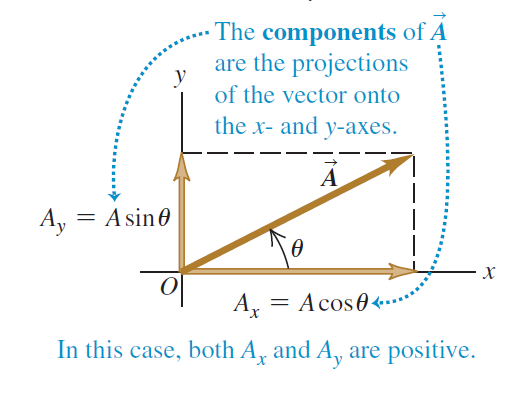
\includegraphics[width=.4\linewidth]{12.png}
	\caption{}
\end{figure}

In the picture above, we have a vector$\vv{A}$ with magnitude $\left|\vv{A}\right|$, so it is easy to find its component on x-axis is $\left|\vv{A}\right|\cos \theta$ and component on y-axis is $\left|\vv{A}\right|\sin \theta$, thus, by vector addition we have:
\begin{equation}\label{E:Converting}
	\vv{A} = \left|\vv{A}\right|\cos \theta \vv{i} + \left|\vv{A}\right|\sin \theta \vv{j}
\end{equation}
Then, we write\footnote{Some book prefer
	$
	\begin{bmatrix}
		\left|\vv{A}\right|\cos \theta	\\
		\left|\vv{A}\right|\sin \theta
	\end{bmatrix}
	$.}\label{f:7}
\begin{equation}\label{E:Coo}
	\vv{A} = 
	\begin{pmatrix}
		\left|\vv{A}\right|\cos \theta	\\
		\left|\vv{A}\right|\sin \theta
	\end{pmatrix}
\end{equation}
Here, let $A_x = \left|\vv{A}\right|\cos \theta, A_y = \left|\vv{A}\right|\sin \theta$, by applying Pythagorean theorem, we have:
\begin{theorem}\label{T:Length} \textbf{(The Magnitude of Vectors)}
	\begin{equation}\label{E:Length}
		\left|\vv{A}\right| = \sqrt{A_x^2 + A_y^2}
	\end{equation}
	It is not hard to see that in xyz-coordinates, the formula would be:
	\begin{equation}\label{E:Length}
		\left|\vv{A}\right| = \sqrt{A_x^2 + A_y^2+ A_z^2}.
	\end{equation}
\end{theorem}

A numerical example
\footnote{The source of the figure is \textit{Mathematics Application and Interpretation HL 2} by Michael Haese, Mark Humphries, Chris Sangwin and Ngoc Vo.}:
\begin{figure}[h]
	\centering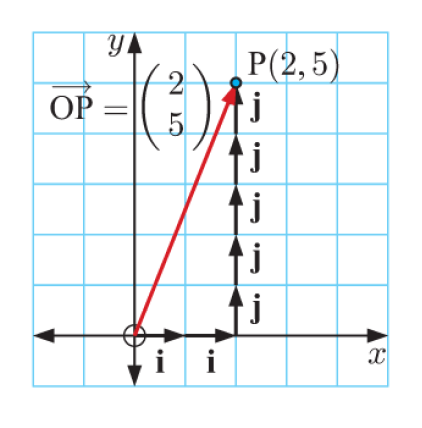
\includegraphics[width=.25\linewidth]{13.png}
	\caption{}
\end{figure}
\begin{align*}
	\text{Here } \vv{OP}=2\vv{i}+5\vv{j}, \text{ hence } \vv{OP} =
	\begin{pmatrix}
		2	\\
		5
	\end{pmatrix}
	\text{ and } \left|\vv{OP}\right| = \sqrt{2^2 + 5^2} = \sqrt{29}.
\end{align*}

What I mean by this subsection is that, when we write a vector as things like $\vv{A}=\begin{pmatrix}
	2	\\
	5
\end{pmatrix}$, what we really mean is that $\vv{A}=2\vv{i}+5\vv{j}$.

\subsection{``Translating"}\label{SS:TRANS}\hfill

We finally made it here. The final jobs are to ``translate" things in section~\ref{S:VGV} into coordinates.

Suppose we have three vectors:
\begin{equation*}
	\vv{a} = 
	\begin{pmatrix}
		a_1	\\
		a_2 \\
		a_3
	\end{pmatrix},\quad
	\vv{b} = 
	\begin{pmatrix}
		b_1	\\
		b_2 \\
		b_3
	\end{pmatrix},\quad
	\vv{c} = 
	\begin{pmatrix}
		c_1	\\
		c_2 \\
		c_3
	\end{pmatrix}
\end{equation*}

\begin{itemize}
	\item $\vv{a} = \vv{b} \Leftrightarrow a_1 = b_1, a_2 = b_2, a_3 = b_3$;
	\item $-\vv{a}=-\begin{pmatrix}
		a_1	\\
		a_2 \\
		a_3
	\end{pmatrix}=\begin{pmatrix}
	-a_1	\\
	-a_2 \\
	-a_3
	\end{pmatrix}$
	\item $\vv{a}+\vv{b} = \begin{pmatrix}
		a_1 + b_1	\\
		a_2 + b_2 \\
		a_3 + b_3
	\end{pmatrix}$
\end{itemize}

Let me prove the third one to you:
\begin{align*}
	\vv{a}+\vv{b} &= a_1 \vv{i} + a_2 \vv{j} + a_3 \vv{k} + b_1 \vv{i} + b_2\vv{j} + b_3\vv{k}\\
				  &= (a_1 + b_1) \vv{i} + (a_2 + b_2) \vv{j} + (a_3 + b_3)\vv{k}\\
				  &= \begin{pmatrix}
				  	a_1 + b_1	\\
				  	a_2 + b_2 \\
				  	a_3 + b_3
				  \end{pmatrix}
\end{align*}

The proof of other results usually follow the same idea, so I will just list the result here now:
\begin{itemize}
	\item $\vv{a}\parallel \vv{b} \Leftrightarrow a_1 = \lambda b_1, a_2 = \lambda b_2, a_3 = \lambda b_3$
	\item $\vv{a}\cdot \vv{b} = a_1b_1 + a_2b_2 + a_3b_3$
	\item $\left|\vv{a}\right| = \sqrt{\vv{a}\cdot \vv{a}} = \sqrt{a_1^2 + a_2^2 + a_3^2}$
	\item By the way, if we want to find a unit vector whose direction is the same as $\vv{a}$, we can have $\displaystyle \frac{1}{\left|\vv{a}\right|}\vv{a}$
	\item $\cos \theta =\displaystyle \frac{a_1b_1 + a_2b_2 + a_3b_3}
	{\sqrt{a_1^2 + a_2^2 + a_3^2}\sqrt{b_1^2 + b_2^2 + b_3^2}}$
	\item $\vv{a} \perp \vv{b} \Leftrightarrow a_1b_1 + a_2b_2 + a_3b_3=0$
\end{itemize}

The vector product or the cross product is a little bit hard:
\begin{align*}
	\vv{a}\times \vv{b} &= (a_1 \vv{i} + a_2 \vv{j} + a_3 \vv{k}) \times (b_1 \vv{i} + b_2\vv{j} + b_3\vv{k})\\
	                    &= a_1b_1 \vv{i}\times\vv{i} + a_1b_2 \vv{i}\times\vv{j} + a_1b_3 \vv{i}\times\vv{k}\\
	                    &\qquad +a_2b_1 \vv{j}\times\vv{i} + a_2b_2 \vv{j}\times\vv{j} + a_2b_3 \vv{j}\times\vv{k}\\
	                    &\qquad\quad +a_3b_1 \vv{k}\times\vv{i} + a_3b_2 \vv{k}\times\vv{j} + a_3b_3 \vv{k}\times\vv{k}
\end{align*}
Please notice that, by applying definition~\ref{D:TVP} and Anticommutative law~\ref{T:AC}, we have:
\[
\begin{array}{c}
	\vv{i}\times\vv{i} = \vv{0}, \vv{j}\times\vv{j} = 0, \vv{k}\times\vv{k} = 0\\
	\vv{i}\times\vv{j} = \vv{k}, \vv{j}\times\vv{i} = -\vv{k}\\
	\vv{i}\times\vv{k} = -\vv{j}, \vv{k}\times\vv{i} = \vv{j}\\
	\vv{j}\times\vv{k} = \vv{i}, \vv{k}\times\vv{j} = -\vv{i}
\end{array}
\]
So keep our calculation, we will have:
\begin{align*}
	\vv{a}\times \vv{b} &= a_1b_2 \vv{k} - a_1b_3\vv{j} - a_2b_1\vv{k} + a_2b_3\vv{i} +a_3b_1\vv{j} - a_3b_2\vv{i}\\
	&=(a_2b_3-a_3b_2)\vv{i} + (a_3b_1-a_1b_3)\vv{j} + (a_1b_2-a_2b_1)\vv{k}\\
	&=
	\begin{pmatrix}
		a_2b_3-a_3b_2	\\
		a_3b_1-a_1b_3 \\
		a_1b_2-a_2b_1
	\end{pmatrix}
\end{align*}

It is hard to remember this result, but if know determinants, then we can actually write it in another way:
\begin{equation}
	\vv{a}\times \vv{b} =
	\begin{vmatrix}
		\vv{i} &\vv{j} &\vv{k}\\
		a_1 & a_2 & a_3\\
		b_1 & b_2 & b_3
	\end{vmatrix}
\end{equation}


\subsection{Triple Product}\label{SS:CTP}\hfill

We have so called triple product. that is $\vv{c}\cdot (\vv{a}\times\vv{b})$ or $(\vv{a}\times\vv{b})\cdot \vv{c}$ (they are the same, because dot product has commutative law):
\begin{definition}\label{D:TP} \textbf{(Triple Product)}\hfill
	For the value of the triple product, we have:
	\begin{equation}
		\vv{c}\cdot (\vv{a}\times\vv{b}) = \left|\vv{c}\right|\left|(\vv{a}\times\vv{b})\right|\cos \psi
	\end{equation}
	Here, $\psi$ is the angle between $\vv{c}$ and $(\vv{a}\times\vv{b})$. Or, in coordinate, using determinant, we have:
	\begin{equation}
		\vv{c}\cdot (\vv{a}\times\vv{b}) =
		\begin{vmatrix}
			c_1 & c_2 & c_3\\
			a_1 & a_2 & a_3\\
			b_1 & b_2 & b_3
		\end{vmatrix}
	\end{equation}
	The key thing is that there is a geometric meaning of triple product, its absolute value is the volume of the parallelepiped\footnote{The source of the figure is 《解析几何(第三版)》by 丘维声.}\label{f:Parallelepiped}:
	\begin{figure}[h]
		\centering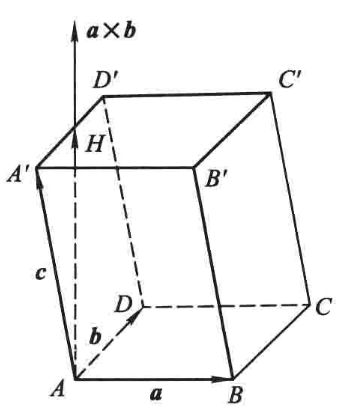
\includegraphics[width=.2\linewidth]{15.png}
		\caption{}
	\end{figure}
	
	This is because $\left|\vv{c}\right|\cos \psi$ is actually the height of the parallelepiped, while $\left|(\vv{a}\times\vv{b})\right|$ is the area of the base of the parallelepiped. Hence it is obvious to see it.
\end{definition}

\newpage
\section{$\ ^\ast$Epilogue}\label{S:EPI}

\subsection{Inequalities}\label{SS:INEQ}\hfill

Using dot product (scalar product) we can prove two famous and important inequalities:
\begin{theorem}\label{Schwarz} \textbf{(Cauchy-Schwarz Inequalities)}
	\begin{equation}\label{E:Schwarz}
		\sum_{i=1}^{3} x_iy_i \le \sqrt{\sum_{i=1}^{3} x_i^2}\sqrt{\sum_{i=1}^{3} y_i^2}
	\end{equation}
\end{theorem}

\begin{proof}
	Let $\vv{x}=\begin{pmatrix}
		x_1\\
		x_2\\
		x_3
	\end{pmatrix}$
	and $\vv{y}=\begin{pmatrix}
		y_1\\
		y_2\\
		y_3
	\end{pmatrix}$ We have
	\begin{align*}
		\cos \theta = \frac{x_1y_1 + x_2y_2 + x_3y_3}
		{\sqrt{x_1^2 + x_2^2 + x_3^2}\sqrt{y_1^2 + y_2^2 + y_3^2}}
	\end{align*}
	Clearly, $\cos \theta \le 1$ Hence
	\begin{equation*}
		\frac{x_1y_1 + x_2y_2 + x_3y_3}
		{\sqrt{x_1^2 + x_2^2 + x_3^2}\sqrt{y_1^2 + y_2^2 + y_3^2}} \le 1
	\end{equation*}
	Which is what we want:
		\begin{equation*}
		\sum_{i=1}^{3} x_iy_i \le \sqrt{\sum_{i=1}^{3} x_i^2}\sqrt{\sum_{i=1}^{3} y_i^2}
	\end{equation*}
\end{proof}

Maybe you are more familiar with this inequality when we are in 2-D plane, but the result and proof are pretty similar. Actually, the generalized version of it should be:
\begin{equation}\label{E:GSchwarz}
	\sum_{i=1}^{n} x_iy_i \le \sqrt{\sum_{i=1}^{n} x_i^2}\sqrt{\sum_{i=1}^{n} y_i^2}
\end{equation}
You can prove it using the similar method here as long as you think or ``believe" there is a angle in $n$ dimension space. Otherwise, you shall use some other method. I put this at here because I usually forget this important inequality, but with vector, it is quite easy to remember, just:
\begin{equation}\label{SchwarzV}
	\vv{x}\cdot \vv{y} \le \left|\vv{x}\right|\left|\vv{y}\right|
\end{equation}

Another import inequality is:
\begin{theorem}\label{TRI} \textbf{(Triangle Inequality)}
	\begin{equation}\label{E:TRI}
		\left|\vv{x}+\vv{y}\right| \le \left|\vv{x}\right| + \left|\vv{y}\right|
	\end{equation}
\end{theorem}

\begin{proof}
	We have:
	\begin{align*}
		(\left|\vv{x}+\vv{y}\right|)^2 &= (\vv{x}+\vv{y})\cdot (\vv{x}+\vv{y})\\
		 &= \left|\vv{x}\right|^2 + 2\vv{x}\cdot \vv{y} + \left|\vv{x}\right|^2\\
		 &\le \left|\vv{x}\right|^2 + 2\left|\vv{x}\right|\left|\vv{y}\right| + \left|\vv{x}\right|^2\\
		 &= (\left|\vv{x}\right| + \left|\vv{y}\right|)^2
	\end{align*}
	Hence, we have
	\begin{equation*}
		(\left|\vv{x}+\vv{y}\right|)^2 \le (\left|\vv{x}\right| + \left|\vv{y}\right|)^2
	\end{equation*}
	Notice that both $\left|\vv{x}+\vv{y}\right|$ and $\left|\vv{x}\right| + \left|\vv{y}\right|$ are non-negative numbers, and we have a trivial result that $a^2 \le b^2$ then $a < b$ provided $a \ge 0, b\ge 0$, so we have:
	\begin{equation*}
		\left|\vv{x}+\vv{y}\right| \le \left|\vv{x}\right| + \left|\vv{y}\right|
	\end{equation*}
\end{proof}
Forget about the proof for a second, notice that this inequality just said that \textbf{the length of one side of a triangular can not be longer than the sum of the length of the other two sides} (See in Figure~\ref{F:ADD}). Which you shall have learned in your young age.

\subsection{Direction Cosine}\label{SS:DC}\hfill

Some book might also introduce the concepts direction angles and direction cosine:
\begin{definition}\label{D:DC} \textbf{(Direction Angles and Direction Cosine)}
	The \textbf{direction angles} of a vector $\vv{a}$ is the angle between $\vv{a}$ and $\vv{i}, \vv{j}, \vv{k}$ i.e. the angle between the vector and the three positive coordinate axes. \textbf{Commonly, they will be denoted by $\alpha \text{(between x-axis)}, \beta\text{(between y-axis)}, \gamma\text{(between z-axis)}$}. And the \textbf{direction cosines} (or directional cosines) of a vector are the cosines of the angles between the vector and the three positive coordinate axes.
\end{definition}

Using dot product, the direction cosines are not hard to calculate, let $\vv{a}=\begin{pmatrix}
	x\\
	y\\
	z
\end{pmatrix}$:
\begin{align}\label{E:DC}
	\cos \alpha = \frac{\vv{a}\cdot \vv{i}}{\left|\vv{a}\right|\left|\vv{i}\right|}
	=\frac{x}
	{\sqrt{x^2 + y^2 + z^2}}\\
	\cos \beta = \frac{\vv{a}\cdot \vv{j}}{\left|\vv{a}\right|\left|\vv{j}\right|}
	=\frac{y}
	{\sqrt{x^2 + y^2 + z^2}}\\
	\cos \gamma = \frac{\vv{a}\cdot \vv{k}}{\left|\vv{a}\right|\left|\vv{k}\right|}
	=\frac{z}
	{\sqrt{x^2 + y^2 + z^2}}
\end{align}

Two interesting things here, first:
\begin{equation}\label{E:CCC1}
	{\cos \alpha}^2 + {\cos \beta}^2 + {\cos \gamma}^2 = 1
\end{equation}
Second, we have said in section~\ref{SS:TRANS} that to find a unit vector whose direction is the same as $\vv{a}$, we just need $\displaystyle \frac{1}{\left|\vv{a}\right|}\vv{a}$, here it should be:
\begin{equation*}
	\frac{1}{\left|\vv{a}\right|}\vv{a} = \frac{1}{\sqrt{x^2 + y^2 + z^2}}\begin{pmatrix}
		x\\
		y\\
		z
	\end{pmatrix}
	= \begin{pmatrix}
		\frac{x}
		{\sqrt{x^2 + y^2 + z^2}}\\
		\frac{y}
		{\sqrt{x^2 + y^2 + z^2}}\\
		\frac{z}
		{\sqrt{x^2 + y^2 + z^2}}
	\end{pmatrix}
\end{equation*}

Do you see that, we just find that:
\begin{equation}\label{E:UCCC}
	\text{The unit vector for $\vv{a}$: }\frac{1}{\left|\vv{a}\right|}\vv{a} = \begin{pmatrix}
		\cos \alpha\\
		\cos \beta\\
		\cos \gamma
	\end{pmatrix}
\end{equation}


%% 1. 不要忘记label
%
%\section{Some General Definitions}\label{S:SGD}
%
%% 2. \hfill
%
%\begin{definition*}\hfill
%	\begin{itemize}
	%		\item $\mathbb{R}^n$: The collection of all column vectors with $n$ components;
	%		we call it ``n-space"
	%		\item $T: \mathbb{R}^n \mapsto \mathbb{R}^m$: A rule associates each element in set $\mathbb{R}^n$.
	%		with one and only one element in set $\mathbb{R}^m$. We call it \textbf{\emph{map or transformation from $\mathbb{R}^n$ to $\mathbb{R}^m$}}. When $n=m$, we call it
	%		an \emph{operator} on $\mathbb{R}^n$.
	%	\end{itemize}
%\end{definition*}
%
%% 3. \displaystyle
%
%$A = \displaystyle \left[\begin{matrix}1 & 2\\3 & 2\\1 & -1\end{matrix}\right]$
%
%% 4. 一行多个公式
%
%\begin{align*}
%	&\text{a)}\ \lim_{x\to 0}\frac{\sin 2\theta}{\theta},
%	&       &\text{b)}\ \lim_{x\to 0} \frac{\sin \frac{x}{2}\cos x}{x}\\
%	&\text{c)}\ \lim_{x\to 0} \frac{\sin x \sin 4x}{x^2},
%	&       &\text{d)}\ \lim_{x\to 0}\frac{\tan x - \sin x}{x^3}\\
%\end{align*}
%
%% 5. 图片
%
%\begin{minipage}{.5\textwidth}
%	\centering
%	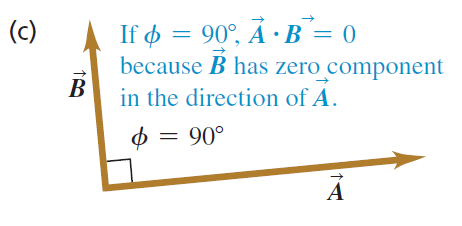
\includegraphics[width=.9\linewidth]{6.png}
%	\captionof*{figure}{(a)}
%\end{minipage}%
%\begin{minipage}{.5\textwidth}
%	\centering
%	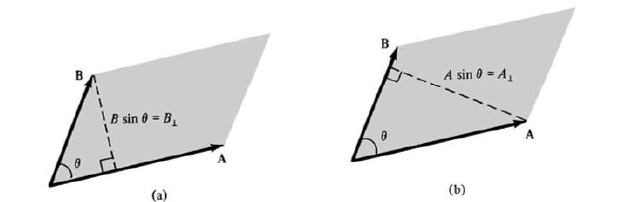
\includegraphics[width=.9\linewidth]{7.png}
%	\captionof*{figure}{(b)}
%\end{minipage}
%
%\begin{figure}[h]
%	\centering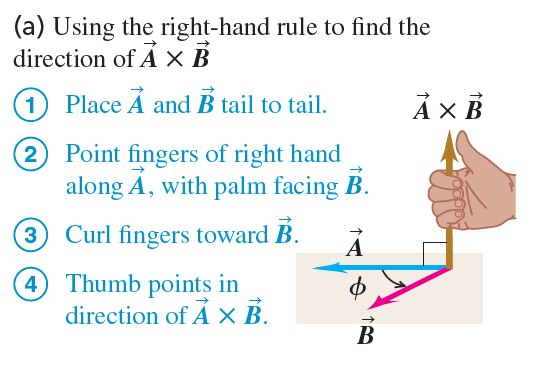
\includegraphics[width=.5\linewidth]{8.png}
%	\caption*{(c)}
%\end{figure}

% 6. 超链接
%\href{https://en.wikipedia.org/wiki/Trigonometric_functions}{the Wikipedia website of trigonometric functions}


%BEGIN_FOLD
%\begin{thebibliography}{99}
%
%\end{thebibliography}
%ENDFOLD
\end{document}

%BEGIN_FOLD
%Papers:
%
%\bibitem{xxx}
%   author, \emph{title}, journal \textbf{volume} 
%    (year), pp.~pages.
%
%Books:
%
%\bibitem{xxx}
%   author, \emph{title}, publisher, address, year.
%
%\bibitem{xxx}
%   author, \emph{title}, series, vol.~volume, 
%    publisher, address, edition, date.
%
%\bibitem{xxx}
%   editor, ed., \emph{title}, publisher, address, year.
%
%Papers in books:
%
%\bibitem{xxx}
%   author, \emph{title}, book title, publisher, 
%    year, pp~pages.
%
%\bibitem{xxx}
%   author, \emph{title}, book title (editor, ed.), 
%    vol.~volume, publisher, publisher address, date, 
%    pp.~pages.
%
%Theses:
%
%\bibitem{xxx}
%   author, \emph{title}, Ph.D. thesis, university, year.
%
%Tech reports:
%
%\bibitem{xxx}
%   author, \emph{title}, tech. report, university, year.
%
%Research notes:
%
%\bibitem{xxx}
%   author, \emph{title}, Research Note number,  
%    university, location, date, research paper in
%    preparation. 
%
%Conference proceedings:
%
%\bibitem{xxx}
%   author, \emph{title}, conference title (location, 
%    year).
%
%\bibitem{xxx}
%   author, \emph{title}, conference title, year
%    (editor, ed.), vol.~volume, publisher, address, 
%    pp.~pages. 
%  
%Abstracts:
%
%\bibitem{xxx}
%   author, \emph{title}, Abstract: journal, volume, 
%    year.
%END_FOLD
